% 2006 Chongqing science q19: pyramid P-ABCD schematic, .6pt, gray, 12pt
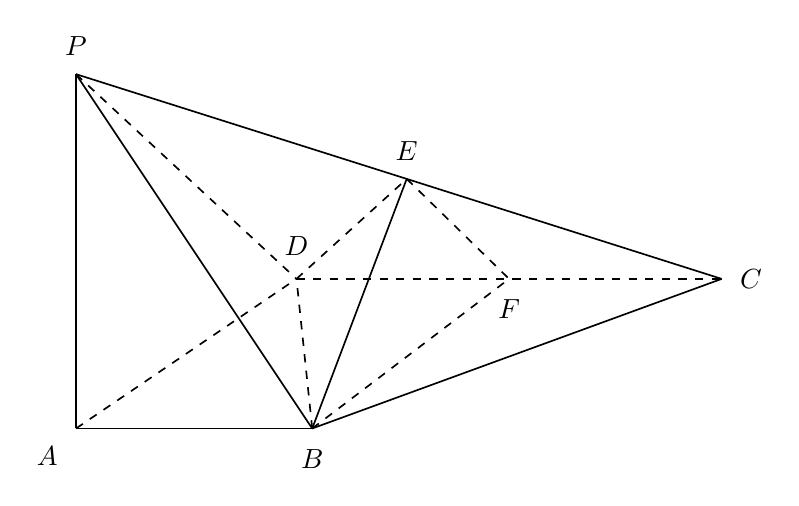
\begin{tikzpicture}[line width=.6pt, font=\normalsize]
\coordinate (P) at (0,4.5);
\coordinate (A) at (0,0);
\coordinate (B) at (3,0);
\coordinate (D) at (2.8,1.9);
\coordinate (E) at (4.2,3.17);
\coordinate (F) at (5.5,1.9);
\coordinate (C) at (8.2,1.9);
% solid visible edges
\draw[solid] (P) -- (A);
\draw[solid] (A) -- (B);
\draw[solid] (B) -- (C);
\draw[solid] (P) -- (E);
\draw[solid] (E) -- (C);
\draw[solid] (P) -- (B);
\draw[solid] (B) -- (E);
% hidden edges
\draw[dashed] (A) -- (D);
\draw[dashed] (P) -- (D);
\draw[dashed] (B) -- (D);
\draw[dashed] (D) -- (E);
\draw[dashed] (D) -- (C);
\draw[dashed] (B) -- (F);
\draw[dashed] (E) -- (F);
% labels offset from strokes
\node[above=3pt] at (P) {$P$};
\node[below left=3pt] at (A) {$A$};
\node[below=4pt] at (B) {$B$};
\node[above=5pt] at (D) {$D$};

\node[above=3pt] at (E) {$E$};
\node[below=4pt] at (F) {$F$};
\node[right=3pt] at (C) {$C$};
\end{tikzpicture}